\documentclass{beamer}
\usepackage{movie15}
\usetheme{AnnArbor}
\usecolortheme{dolphin}
\setbeamercolor*{frametitle}{bg=white,fg=structure.fg}
\title{Exploring the parallelisation of the Large Eddy Simulation using MPI and
the Glasgow Model Coupling Framework}
\author{Gordon Reid - 1002536r}
\date{April 22, 2015}
\newif\ifplacelogo
\placelogofalse
\logo{\ifplacelogo
\includegraphics[width=2cm]{images/ARCHIE-WeSt_logo1.jpg}\vspace{180pt}\fi}
\begin{document}
\frame{\titlepage}
\frame{\tableofcontents}
\section{LES}
\subsection{What is the LES?}
\frame{
    \frametitle{What is the LES?}
    \begin{itemize}
        \item Developed by the Disaster Prevention Research Institute at Kyoto University
        \item Large Eddy Simulation models turbulent flows in urban environments
        \item Geographical Information System data for terrain and building data
        \item High resolution over mesoscale area (100s of km)
        \item Poisson equation solver for linear system of equations using successive over relaxation
        \item Operates over 3D area, outputs 4D arrays to netCDF files
    \end{itemize}
}
\frame{
    \frametitle{What is the LES?}
    \includemovie[poster,repeat,controls,text={Click to play}]
                 {6cm}{4cm}{videos/pressure_at_75_over_t.avi}
    \begin{itemize}
        \item Video shows evolution of pressure over time for a 2D slice of area
        \item Data can be visualised like this or used as input to another model
        \item Originally in FORTRAN 77, automatically ported to Fortran 95
        \item Single-threaded, candidate for parallelisation
    \end{itemize}
}
\subsection{Parallelisation Techniques}
\frame{
    \frametitle{Parallelisation Techniques}
    \begin{itemize}
        \item Parallelisation reduces runtime for fixed size area
        \item Performance improvement can be used to simulate larger areas
        \item Using MPI for shared- and distributed-memory parallelism
        \item Using GMCF for shared-memory parallelism
        \item MPI performance acts as baseline to compare GMCF with
        \item GMCF distributed-memory ability is future work
    \end{itemize}
}
\frame{
    \frametitle{Parallelisation Techniques}
    \includegraphics[width=0.5\textwidth]{images/mpiLESGrid.pdf}
    \begin{itemize}
        \item LES instances organised into 2D grid, each taking slice of total area
        \item Processes communicate to distribute and gather whole arrays
        \item At each time step, side flows and halos need to be exchanged
        \item Halos require up to eight messages: four edges and four corners
        \item Also global reductions to get the min, max, and sum of scalars
    \end{itemize}
}
\section{GMCF}
\subsection{What is GMCF?}
\frame{
    \frametitle{What is GMCF?}
    \begin{itemize}
        \item New model coupling framework: Glasgow Model Coupling Framework
        \item Model coupling allows to separate applications to interact
        \item LES can be coupled to the Weather Research and Forecasting model
        \item Shown to improve accuracy of results
        \item Existing model coupling frameworks can require a lot of work to use
        \item GMCF aims to automate some of the model coupling work
        \item Existing frameworks not multicore or heterogeneous aware, GMCF is
        \item GMCF uses a load balancing technique to limit node communication
    \end{itemize}
}
\subsection{GMCF Architecture}
\frame{
    \frametitle{GMCF Architecture}
    \includegraphics[width=0.5\textwidth]{images/gmcfArchitecture.png}
    \begin{itemize}
        \item GMCF uses threads, one per model instance
        \item Each instance has its own GMCF Tile that holds all data for it
        \item GMCF has a concept of packets, instances communicate via packets
        \item Packets for requesting data, sending pointers to data, and more
        \item Received packets are demultiplexed into per type per sender FIFOs
    \end{itemize}
}
\placelogotrue
\section{Evaluation}
\frame{
    \frametitle{Evaluation}
    \begin{itemize}
        \item MPI and GMCF shared-memory evaluation on togian
        \item togian has 64 cores across 4 sockets
        \item Performance scaling as instance count grew from 1 to 64
        \item MPI distributed-memory evaluation on ARCHIE
        \item ARCHIE is a cluster with thousands of cores
        \item Evaluation used up to 12 nodes (144 cores)
        \item Performance scaling as each additional node added
        \item Fixed area test where total area was 150x150x90
        \item Expanding area test where each instance had 150x150x90 area
    \end{itemize}
}
\placelogofalse
\subsection{MPI Shared-memory evaluation}
\frame{
    \frametitle{MPI Shared-memory evaluation}
    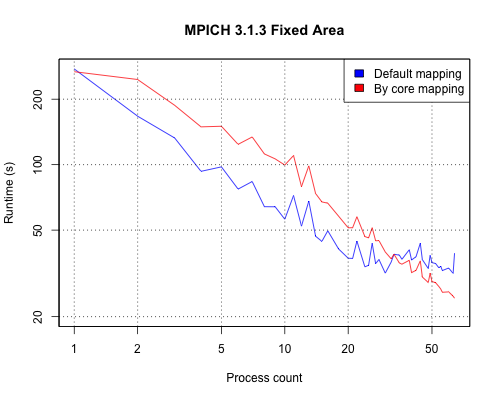
\includegraphics[width=0.5\textwidth]{images/MPICH313-fixed-area.png}
    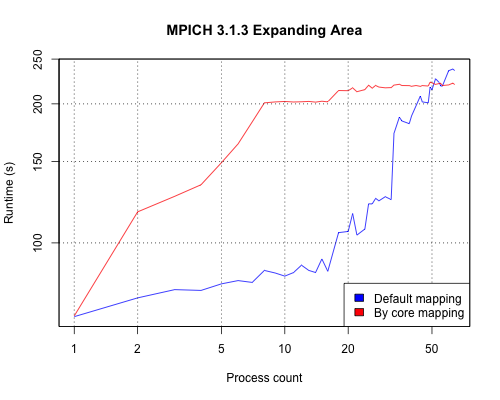
\includegraphics[width=0.5\textwidth]{images/MPICH313-expanding-area.png}
    \begin{itemize}
        \item Default mapping - round robin across sockets
        \item By core mapping - sequential core assignment
        \item MPICH and OpenMPI tested, both performed similarly
        \item Fixed area has linear scaling: 7x improvement over 64 cores
        \item Expanding area runtime settles to 220 seconds
    \end{itemize}
}
\subsection{GMCF Shared-memory evaluation}
\frame{
    \frametitle{GMCF Shared-memory evaluation}
    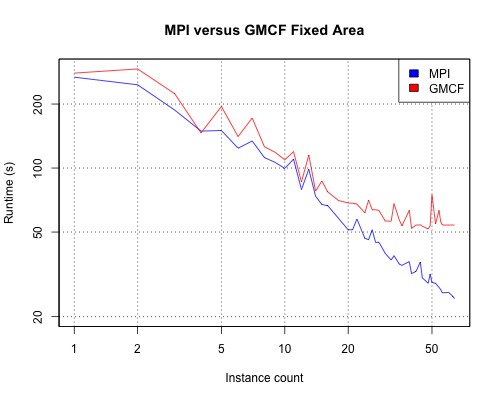
\includegraphics[width=0.5\textwidth]{images/GMCF-MPI-fixed-area.png}
    \includegraphics[width=0.5\textwidth]{images/GMCF-MPI-expanding-area.png}
    \begin{itemize}
        \item Fixed area scales well initially, levels out around 2x slower than MPI
        \item Expanding area performance very similar to MPI, scales well.
        \item Performance competitive with MPI even with MPIs maturity
        \item Smaller transfers need more work to improve performance
    \end{itemize}
}
\subsection{MPI Distributed-memory evaluation}
\frame{
    \frametitle{MPI Distributed--memory evaluation}
    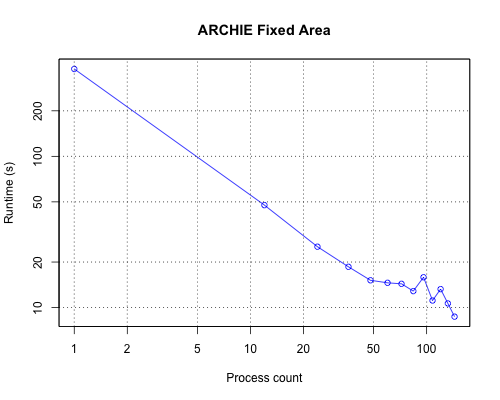
\includegraphics[width=0.5\textwidth]{images/ARCHIE-fixed-area.png}
    \includegraphics[width=0.5\textwidth]{images/ARCHIE-expanding-area.png}
    \begin{itemize}
        \item Fixed area shows linear scaling. 48 cores offers 25x improvement
        \item 144 cores offers 43.5x improvement but individual areas very small
        \item Expanding area shows runtime levels out around 220 seconds
        \item Variation in runtime caused by varying load in ARCHIE overall
    \end{itemize}
}
\section{GMCF Performance Improvements}
\frame{
    \frametitle{GMCF Performance Improvements}
    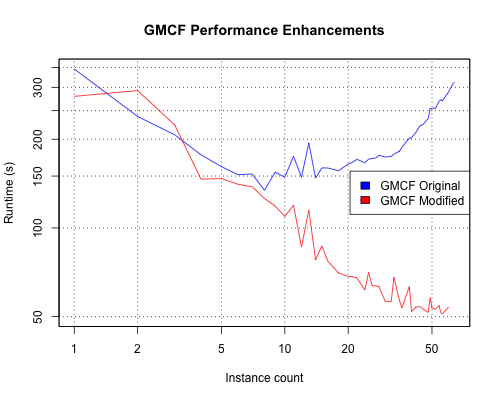
\includegraphics[width=0.5\textwidth]{images/GMCF-before-after-fixed-area.png}
    \begin{itemize}
        \item GMCF originally had `bathtub' shaped graph as thread count grew
        \item Global reductions primary cause of performance problems
        \item Spin locks on FIFOs improved performance by 20\%
        \item Thread pinning reduced runtime by 17\%
        \item Preemptive data sending reduced runtime by 30\%
        \item More granular FIFOs reduced runtime by 20\%
    \end{itemize}
}
\section{Conclusion and Future Work}
\frame{
    \frametitle{Conclusion and Future Work}
    \begin{itemize}
        \item GMCF's performance is competitive with MPI
        \item GMCF well placed to act as parallelisation and model coupling framework
        \item Future work will add distributed memory parallelism
        \item Automation of model coupling can be extended to include automatic parallelisation
        \item Further performance improvements
        \item MPI LES stable
    \end{itemize}
}
\end{document}
